\documentclass[red]{beamer}

%\usetheme{default}
\usetheme{Darmstadt}
%\usecolortheme{beaver}

\setbeamertemplate{navigation symbols}{} 
\useoutertheme[subsection=false]{miniframes}

%\usepackage{iwona}

\usepackage{amsfonts}
\usepackage{amsmath}
\usepackage{amsthm}
\usepackage{amssymb}
\usepackage{graphicx}

\usepackage[american]{babel}
\usepackage{csquotes}
\usepackage[style=apa,natbib=true,backend=biber]{biblatex}
\DeclareLanguageMapping{american}{american-apa}
\addbibresource{Polarization.bib}
% smaller references
\renewcommand*{\bibfont}{\scriptsize}

\newcommand{\vitem}{\vfill\item}

\usepackage{hyperref}
\ExecuteBibliographyOptions{doi=false}
\newbibmacro{string+doi}[1]{%
  \iffieldundef{doi}{#1}{\href{http://dx.doi.org/\thefield{doi}}{#1}}}
\DeclareFieldFormat{title}{\usebibmacro{string+doi}{\mkbibemph{#1}}}
\DeclareFieldFormat[article]{title}{\usebibmacro{string+doi}{\mkbibquote{#1}}}

\title[Technical Change and Wages]{Technical Change and wages in Australia}
\author{Alex Cooper \\ Honours Candidate \\ Macquarie University}
%\institution[Macquarie University]{Macquarie University}
\date{November 2013}

\setlength{\itemsep}{\fill}

\usepackage[absolute,overlay]{textpos}
\pgfdeclareimage[height=1.4cm]{fg:logo}{logo.pdf}
%\logo{\includegraphics[height=1.4cm]{logo.pdf}}
%\useouterframe{subsection=false}

\begin{document}
%
\begin{frame}[plain]
\titlepage
\begin{textblock*}{\textwidth}(3.2in,3in) 
  \pgfuseimage{fg:logo} 
\end{textblock*} 
\end{frame}

\section{Motivation}

\subsection{Inequality Chart}
\begin{frame}[c]
\frametitle{Motivation: rising wage inequality}
\begin{center}
  \includegraphics[width=\textwidth]{slides_fig/ineq_time.pdf}
\end{center}
\end{frame}

\begin{frame}[c]
\frametitle{Drivers of wage inequality}
Leigh, A. (2013). \emph{Battlers \& Billionaires: The Story of Inequality in Australia.} Black Incorporated.
\begin{enumerate}
\vitem Decline in union coverage
\vitem Falling income taxes
\vitem {\bf Technical change}
\pause
\begin{itemize}
  \vitem Globalization of firms
  \vitem Skill-biased technical change (SBTC)
  \vitem Routinization and labor outsourcing
\end{itemize}
\end{enumerate}
\end{frame}

\begin{frame}[c]
\frametitle{Real cost of computation has decreased exponentially}
\begin{center}
  \includegraphics[width=0.8\textwidth]{slides_fig/nordhaus_2007.pdf}
\end{center}
Price per computation/second, 2006 USD (Nordhaus 2007)
\end{frame}

\subsection{Outline}
\begin{frame}[c]
\frametitle{Question: Does technical change drive inequality?}
Three approaches:
\begin{enumerate}
\vfill\item The `canonical' model of skill-biased technical change (SBTC)
\pause
\vfill\item ICT investment and occupational groups
\pause
\vfill\item Assignment approach: `task content' of occupations
\end{enumerate}
\end{frame}

\section{The Canonical Model}
 \subsection{Two types of labor}
\begin{frame}[c]
\begin{center}
  1. The `Canonical' Model
\end{center}
\end{frame}

\begin{frame}[c]
\frametitle{Two types of labor: low-skilled}
\begin{center}
  \includegraphics[width=\textwidth]{slides_fig/low_skill.jpg}
\end{center}
Construction workers at the Rockerfeller Center, NY, 1932
\end{frame}

\begin{frame}[c]
\frametitle{Two types of labor: high-skilled}
\begin{center}
  \includegraphics[width=\textwidth]{slides_fig/high_skill.jpg}
\end{center}
Ester Gerston \& Gloria Gordon program ENIAC, 1946
\end{frame}

\begin{frame}[c]
\frametitle{Production requires high \& low-skilled labor}
\begin{center}
  \vspace{-10pt}
  \makebox[\textwidth]{\includegraphics[width=\paperwidth]{slides_fig/two_types.jpg}}
\end{center}
\end{frame}

\begin{frame}[c]
\frametitle{The `canonical model:' skill-biased technical change}
\begin{center}
  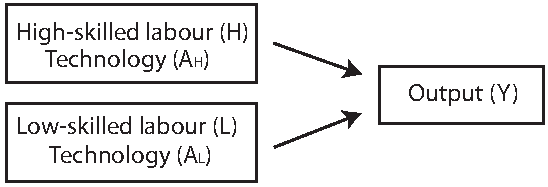
\includegraphics[width=\textwidth]{slides_fig/CES.pdf}
\end{center}
Production function:
\begin{equation*}
  \label{eq:cobbdoug}
  F = \left[\left(A_LL\right)^{\frac{\sigma - 1}{\sigma}}
            + \left(A_HH\right)^{\frac{\sigma - 1}{\sigma}}
          \right]^\frac{\sigma}{(\sigma-1)}
\end{equation*}
We assume $\sigma>1$.
\end{frame}

\begin{frame}
\frametitle{The `canonical model:' comparative statics}
When high-skilled technology is increasing, {\em ceteris paribus},
  \begin{itemize}
  \vitem Increasing inequality, driven by skill demand
  \vitem Rising college/education premium
  \vitem Monotonic wage growth
  \begin{itemize}
    \vitem Across skill spectrum
    \vitem Over time
  \end{itemize}
  
  Importantly: low-skilled wages will never decrease.
  \end{itemize}
% \vspace{1cm}
% \item Empirically successful, e.g.
%   \begin{itemize}
%   \item Katz and Murphy (1992)
%   \item Card and Lemieux (2001)
%   \end{itemize}
% \end{itemize}
\end{frame}

\subsection{Results: wage premium}
\begin{frame}[c]
\frametitle{Monotone wage growth across earnings percentile}
\begin{center}
  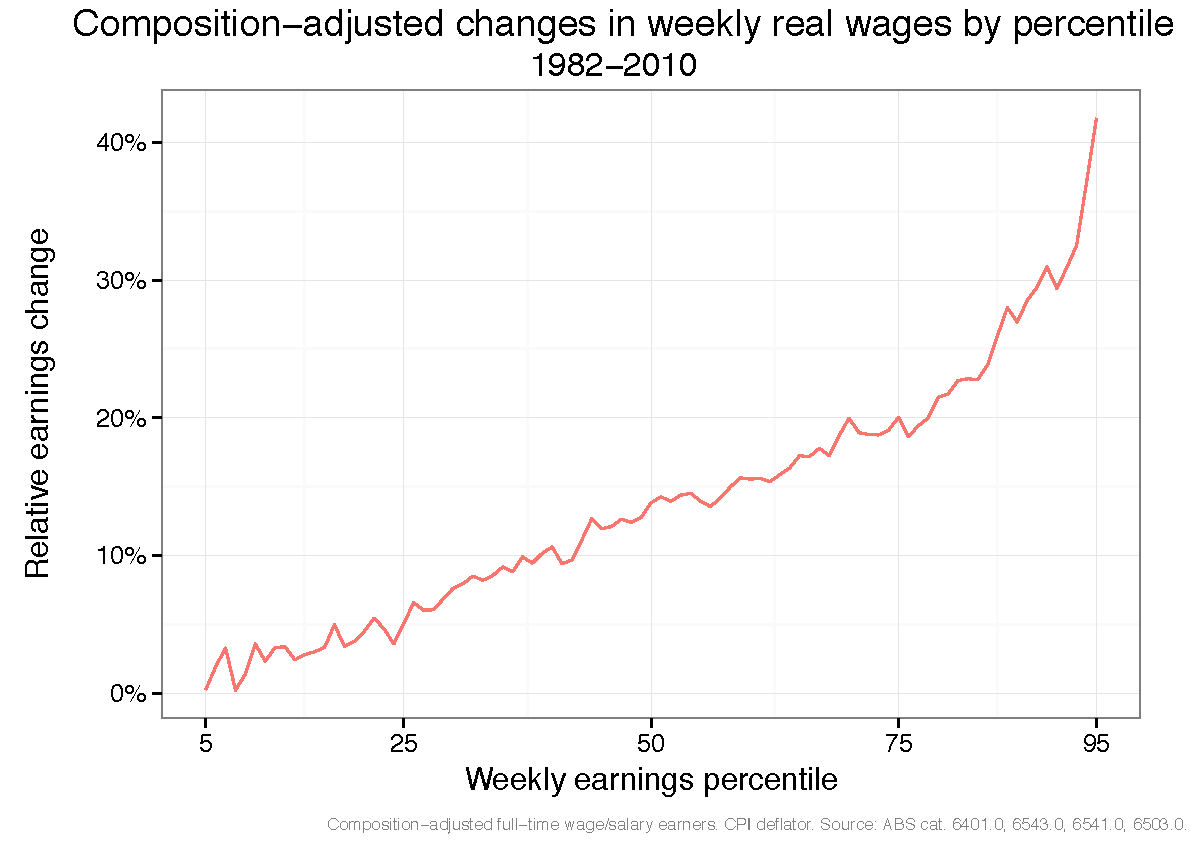
\includegraphics[width=\textwidth]{slides_fig/quantile_growth_percent.pdf}
\end{center}
\end{frame}

\begin{frame}{Non-monotonic wage growth in time}
  \begin{center}
    \includegraphics[width=\textwidth]{slides_fig/wage_change_time.pdf}
  \end{center}
\end{frame}

\begin{frame}
  \frametitle{College wage premium}
  \begin{center}
    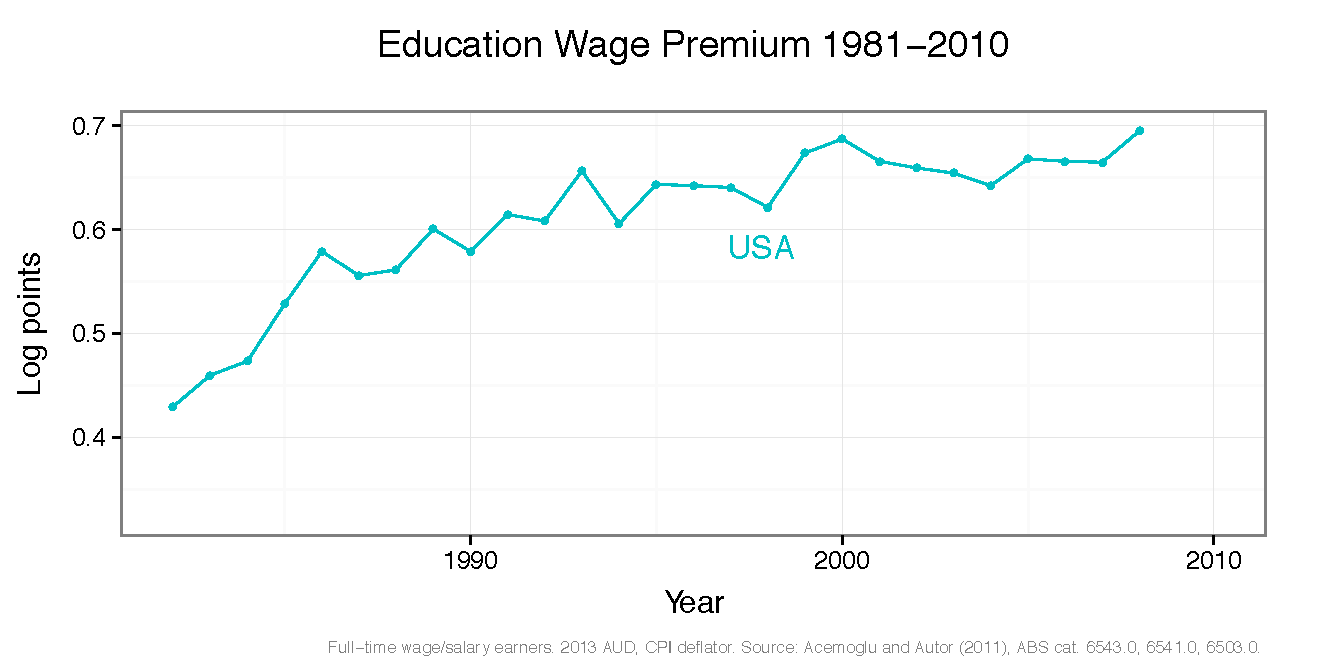
\includegraphics[width=\textwidth]{slides_fig/ed_premium_us.pdf}
  \end{center}
\end{frame}

\begin{frame}
  \frametitle{College wage premium}
  \begin{center}
    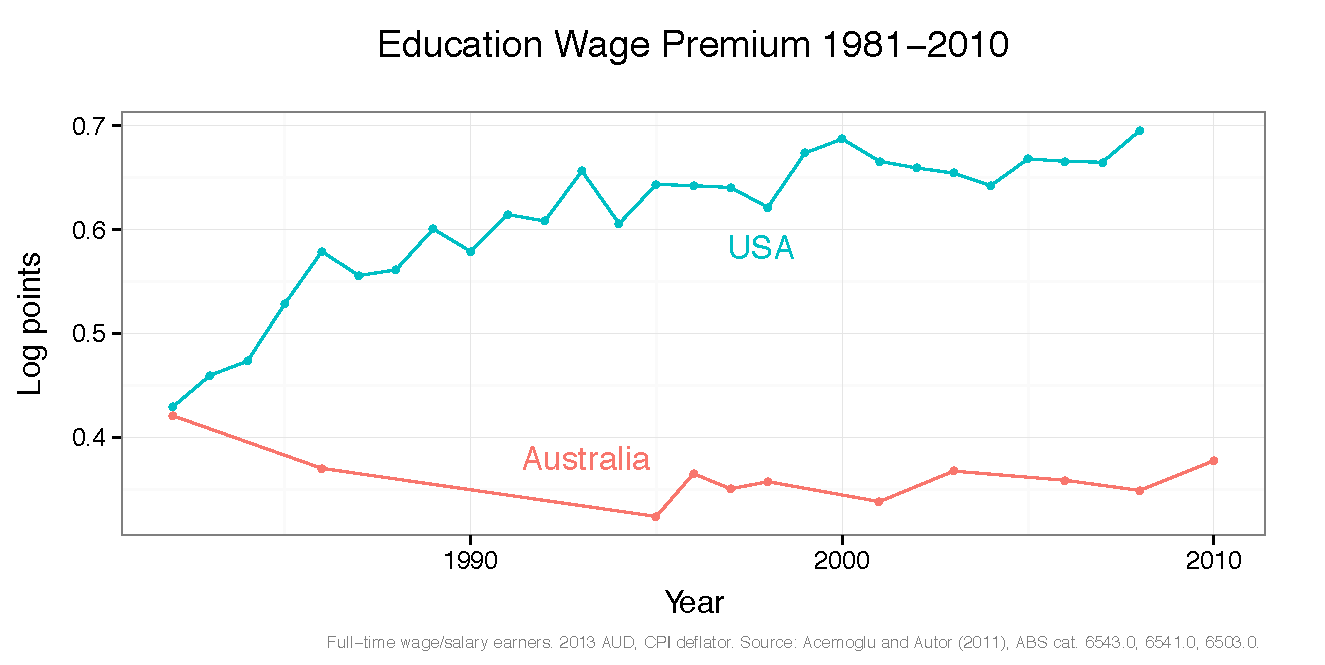
\includegraphics[width=\textwidth]{slides_fig/ed_premium.pdf}
  \end{center}
\end{frame}

\subsection{Results: summary}
\begin{frame}
  \frametitle{Failure of the SBTC model: summary}
  \begin{itemize}
  \vitem No clear `college premium' in Australia (see Coelli 2007)
  \begin{itemize}
  \vitem Education a poor proxy for skills (`credentialism')?
  \vitem Expanding supply of college-educated workers?
  \vitem Does not appear to be driving inequality trend
  \end{itemize}
  \pause
  \vitem Wage growth is non-monotonic
  % \pause
  % \vitem Despite composition adjustment, male and female wage profiles differ
  \end{itemize}
\end{frame}

\subsection{One explanation?}
\begin{frame}{Wage growth by wage percentile and sex}
  \begin{center}
    \includegraphics[width=\textwidth]{slides_fig/quantile_growth_mf.pdf}
  \end{center}
\end{frame}

\begin{frame}{Could job composition explain the trend?}
  \begin{center}
    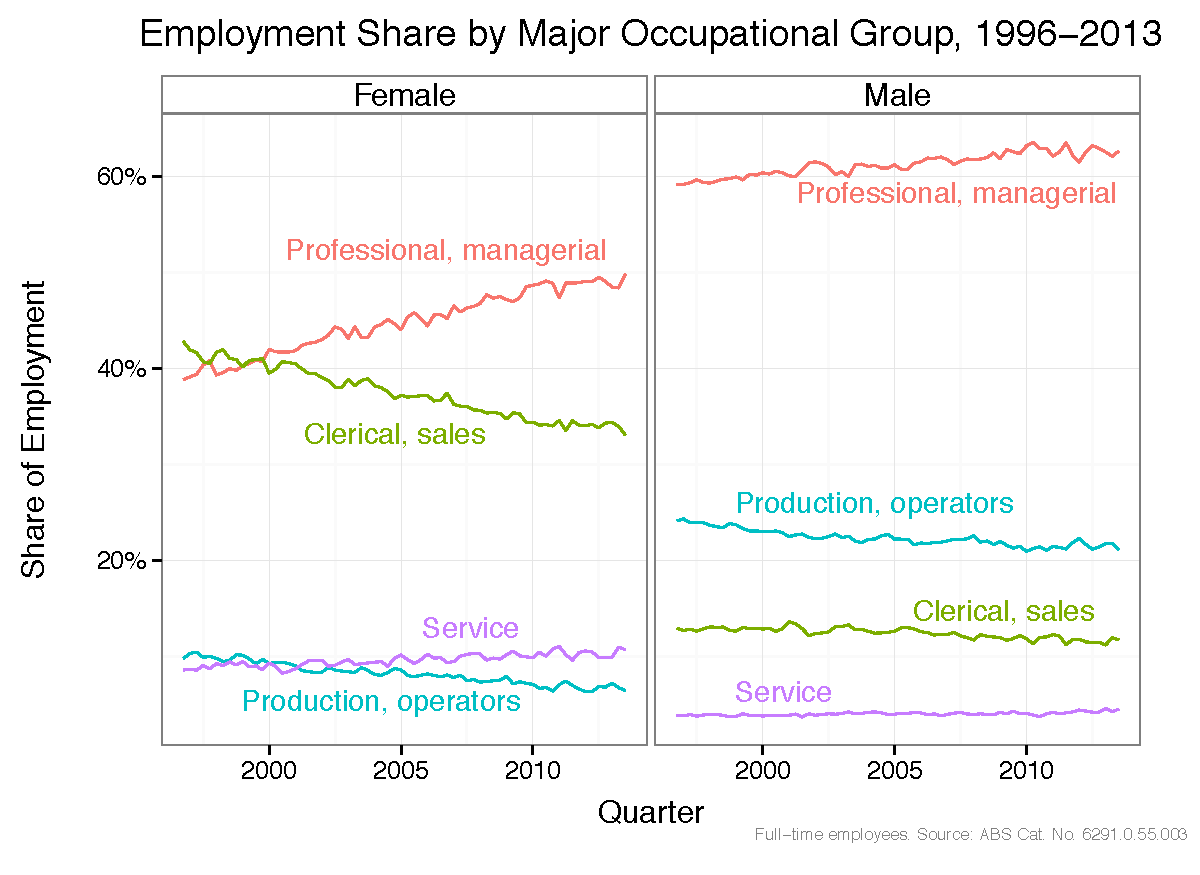
\includegraphics[width=\textwidth]{slides_fig/occ_share_sex.pdf}
  \end{center}
\end{frame}

\section{The `task approach'}
\subsection{Substitutive technology}
\begin{frame}[c]
\begin{center}  2. The Task Approach \end{center}


\vspace{50pt}
(Autor, Levy, and Murnane QJE 2003)
\end{frame}


\begin{frame}[c]
\frametitle{Middle-skilled labor}
\begin{center}
  \includegraphics[width=\textwidth]{slides_fig/three_types_middle.jpg}
\end{center}
A typing pool, Kingsway, London. (Daily Mail)
\end{frame}

\begin{frame}[c]
\frametitle{Production requires three types of labor}
\begin{center}
  \vspace{-10pt}
  \makebox[\textwidth]{\includegraphics[width=\paperwidth]{slides_fig/three_types.jpg}}
\end{center}
\end{frame}

\begin{frame}[c]
\frametitle{Is `skill' an unhelpful concept?}
And can technology {\em replace} as well as assist?
\vfill
\begin{itemize}
\item `Canonical' approach:
\[ \text{capital, labor} \quad \overset{F(\cdot)}{\xrightarrow{\hspace*{1.5cm}}} \quad \text{output}. \]
\begin{itemize}
\item Technology is factor-augmenting
\vfill
\end{itemize}
\pause
\vitem ALM:
\[ \text{capital, labor} \quad \overset{\text{assignment}}{\xrightarrow{\hspace*{1.5cm}}} \quad \text{tasks} \quad \overset{F(\cdot)}{\xrightarrow{\hspace*{1.5cm}}} \quad \text{output}. \]
\begin{itemize}
\item Technology can be complementary or a substitute
\end{itemize}
\end{itemize}
\end{frame}


\begin{frame}[c]
\frametitle{The `task approach'}
\begin{itemize}
\item The canonical approach\\
\begin{center}
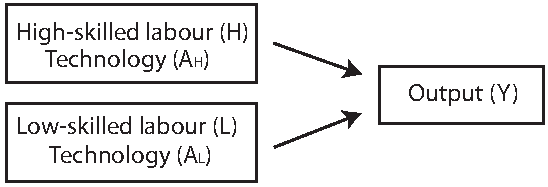
\includegraphics[width=2in]{slides_fig/CES.pdf}
\end{center}
\item The task approach\\
\begin{center}
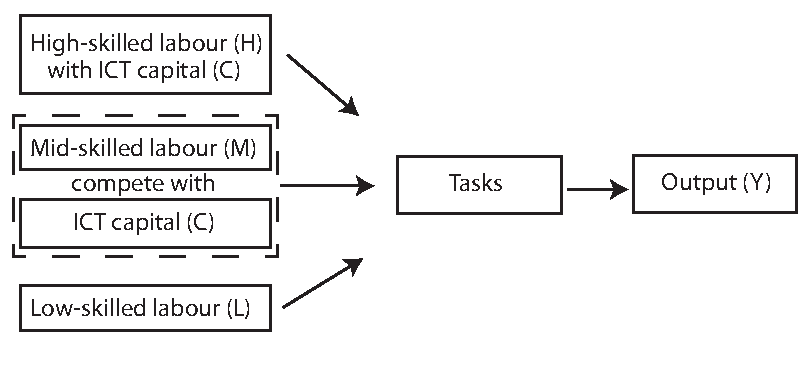
\includegraphics[width=3in]{slides_fig/CES_tasks.pdf}
\end{center}
\end{itemize}
\end{frame}

\subsection{A simple test}
\begin{frame}
\frametitle{The `task approach'}
\begin{itemize}
\vitem Jobs have different task content
\vitem Capital can substitute for only certain `routine' tasks.
  \begin{itemize}
  \item Typically `middle-skill,' like clerical work
  \end{itemize}
\vitem Michaels {\em et al} (2013) expand the canonical model with `middle-skilled' labor
  \begin{itemize}
  \item Three kinds of labor: $H$, $M$, $L$, and ICT capital $C$. 
  \item Capital $C$ and $M$ are perfect substitutes
  \item Middle-skilled workers compete with ICT capital
  \end{itemize}
\end{itemize}
\end{frame}

\begin{frame}[c]
  \frametitle{A simple test (Michaels {\em et al.} 2013)}
Production function with three types of labor and ICT capital $C$:
$$
Y = \left[
  \underbrace{(A_LL)^\frac{\sigma-1}{\sigma}}_{\text{low}}
  +
  \underbrace{(A_MM + C)^\frac{\sigma-1}{\sigma}}_{\text{medium}}
  +
  \underbrace{((A_HH)^\mu + C^\mu)^\frac{\sigma-1}{\mu\sigma}}_{\text{high}}
  \right]^\frac{1}{\sigma-1}
$$
\pause
Comparative statics: if $C$ increases exogenously, then: 
\begin{itemize}
\vitem high-skilled wage share should increase, and 
\vitem medium-skilled wage share should decrease.
\end{itemize}
\end{frame}

\begin{frame}[c]
  \frametitle{ICT capital (equipment) and wage shares by group}
\begin{center}
\includegraphics[width=\textwidth]{slides_fig/wage_share_equipment_skill.pdf}
\end{center}
\end{frame}

\begin{frame}[c]
  \frametitle{Problems with this result}
  \begin{itemize}
    \vitem Model gives only {\em wage share}, not {\em wage}
    \pause
    \vitem ICT investment endogenous, with no obvious instruments
    \pause
    \vitem Tests have low power
    \begin{itemize}
      \item few industry groups
      \item occupational groupings too simplistic
    \end{itemize}
    \pause
    \vitem Conflicting results with other ICT capital measures 
           (software, computer peripherals)
    \pause
    \vitem No obvious way to deflate ICT capital for consistent comparison
  \end{itemize}
\end{frame}

\section{Task Data}
\subsection{Sources}
\begin{frame}
  \frametitle{Task Data}
  \begin{enumerate}
  \vitem Australian occupation coding scheme (ANZSCO, ASCO)
    \begin{itemize}
    \vitem Describe occupations qualitatively
    \vitem Difficult to compare occupations
    \end{itemize}
    \vspace{10pt}
  \vitem O*NET: Occupational task database
    \begin{itemize}
    \vitem Developed by US Department of Labor
    \vitem Details work activities by occupation
    \end{itemize}
  \end{enumerate}
\end{frame}

\begin{frame}
\frametitle{O*NET Data Example}
\begin{table}[htbp]
\begin{tabular}{|p{2cm}|p{1.65cm}|p{1.5cm}|p{1.5cm}|p{1.5cm}|}
\hline
{Job Title} & {Gather Data} & {Analyze Data} & {\small Think Creatively} & {Handle Moving Objects} \\ \hline
{CEOs} & 5.03 & 4.82 & 5.1 & 1.1  \\ \hline
{Economists} & 5.88 & 6.58 & 5.38 & 0.54 \\ \hline
{Dancers} & 3.88 & 1.96 & 4.37 & 2.63 \\ \hline
{Programmers} & 4.91 & 5.05 & 5.96 & 0.44 \\ \hline
{Tellers} & 2.91 & 2.65 & 2.21 & 2.74 \\ \hline
{Surgeons} & 5.72 & 5.49 & 4.67 & 3.62 \\ \hline
{Bakers} & 2.8 & 3.29 & 2.93 & 5.06 \\ \hline
{Receptionists} & 3.1 & 2.45 & 2.54 & 2.88 \\ \hline
{Typists} & 4.35 & 1.52 & 3.9 & 1.43 \\ \hline
\end{tabular}
\caption{O*NET Work Activity Example (Levels, Scale 0--7)}
\label{onetex}
\end{table}
\end{frame}

\begin{frame}[c]
\frametitle{Task Index Construction from O*NET Data}
Example: Automation/Routinization index
\begin{align*}
\text{Index} &= \left(\text{Degree of Automation}\right. \\
&\quad+ \text{Importance of Repeating Same Tasks} \\
&\quad- \text{Structured versus Unstructured Work} \\
&\quad+ \text{Pace Determined by Speed of Equipment} \\
&\quad+ \left.\text{Spend Time Making Repetitive Motions}\right) / 5
\end{align*}

Tasks are normalized to have mean zero and s.d. = 1.
\end{frame}

\begin{frame}[c]
\frametitle{Five Indexes}
The O*NET variables were combined to produce 5 indexes:
\begin{enumerate}
  \vitem `Routinization' indicators
  \begin{itemize}
    \vitem Occupation information content
    \vitem Automation / routinization
  \end{itemize}
  \vitem `Outsourcing' indicators
  \begin{itemize}
    \vitem Lack of face-to-face content
    \vitem Lack of on-site work
    \vitem Lack of decision-making
  \end{itemize}
\end{enumerate}
\end{frame}

\begin{frame}[c]
  \frametitle{Occupational indexes and income}
\begin{center}
\includegraphics[width=\textwidth]{slides_fig/wages_indexes_4digit_pres.pdf}
\end{center}
\end{frame}

\section{Assignment Approach}
\subsection{Assignment Literature}
\begin{frame}
  \frametitle{`Assignment' Approach to Occupational Choice}
  Following Firpo, Fortin, \& Lemieux (2011),
  \begin{itemize}
  \vitem Labor market as Roy model
    \begin{itemize}
    \item Self-selection into occupations by comparative advantage
    \end{itemize}
    \pause
  \vitem At each quantile, decompose wage changes by:
    \[ \Delta \text{ wage quantile} = \text{wage structure effect} + \text{composition effect} \]
  \vitem Caveats:
  \begin{itemize}
  \item our data can only provide point estimates
  \item we can only compare 1981/2001 and 1981/2010.
  \end{itemize}
\end{itemize}
\end{frame}

\begin{frame}[c]
\frametitle{Upper wage distribution affected}
\begin{center}
  \includegraphics[width=\textwidth]{slides_fig/density_as_81.pdf}
\end{center}
\end{frame}

\begin{frame}[c]
  \frametitle{Wage Structure and Composition Effect}
  \includegraphics[width=\textwidth]{../figure/aggregate_decomp.pdf}
\end{frame}

\begin{frame}[c]
  \frametitle{}
  \begin{itemize}
  \vitem 1980s and 1990s was a period of structural wage change across the wage spectrum
  \vitem 2000s saw mostly compositional change, except at top incomes
  \pause
  \vitem How much of the structure effect can be attributed to each task measure?

  We must assume:
  \begin{itemize}
  \vitem Assume tasks contribute to wages additively
  \vitem Also assume task measures don't change over time.
  \end{itemize}
  \vitem Implement decomposition using Oaxaca-Blinder decomposition and RIF regressions
\end{itemize}
\end{frame}

\begin{frame}[c]
  \frametitle{Wage Structure Decomposition}
  \includegraphics[width=\textwidth]{../figure/structure_decomp.pdf}
\end{frame}

\section*{References}

\begin{frame}
  \frametitle{Summary}
  \begin{itemize}
  \vitem Evidence that the work force is `polarising'
  \vitem {\em Type} of work is important
  \vitem Impact of job tasks not uniform across the wage distribution
  \vitem 1980s and 1990s: routinization reduced wages in top income quantiles
  \vitem 2000s: managerial tasks increased wages in top income quantiles
  \vitem Non-customer-facing work is associated with income growth, especially at high incomes
  \end{itemize}
\end{frame}

\begin{frame}
  \begin{center}
    Questions
    \vspace{1cm}

    and
    \vspace{1cm}

    I'd love your feedback.
  \end{center}
\end{frame}

\begin{frame}
\frametitle{References}
%\printbibliography
{ \scriptsize
Acemoglu, D., \& Autor, D. H. (2011). Skills, Tasks and Technologies: Implications for Employment and Earnings. In D. Card \& O. Ashenfelter (Eds.), Handbook of labor economics, volume 4, part b (Chap. 12, Vol. Volume 4, pp. 1043–1171). Elsevier
\vfill

Autor, D. H., Levy, F., \& Murnane, R. J. (2003). “The skill content of recent technological change: An empirical exploration.” The Quarterly Journal of Economics, 118(4), 1279–1333.
\vfill

Card, D., \& Lemieux, T. (2001, May). “Can Falling Supply Explain the Rising Return to College for Younger Men? A Cohort-Based Analysis.” The Quarterly Journal of Economics, 116(2), 705–746
\vfill

Firpo, S., Fortin, N., \& Lemieux, T. (2011). Occupational tasks and changes in the wage structure. Institute for the Study of Labor.
\vfill

Katz, \& Murphy, K. J. (1992). “Changes in Relative Wages, 1963-1987: Supply and Demand Factors.” Quarterly Journal of Economics, 107, 35–78.
}
\end{frame}

% \begin{frame}
%   \begin{center}
%     Spare Slides
%   \end{center}
% \end{frame}

\end{document} 
